\documentclass[11 pt]{article}

\usepackage[margin=1in]{geometry}

\usepackage{parskip}

\usepackage{amsmath}
\usepackage{amssymb}

\usepackage{graphicx}

\usepackage{array}
\usepackage{booktabs}

\usepackage{microtype}

\usepackage{siunitx}
\usepackage{xspace}

\usepackage{setspace}
% \doublespacing

% \usepackage[compact]{titlesec}

\usepackage[]{appendix}




% \usepackage{newtxtext}
% \usepackage{newtxmath}

% Code packages 
	\usepackage[dvipsnames]{xcolor}

	\usepackage{listings}
	\usepackage{color}

	\definecolor{dkgreen}{rgb}{0,0.3,0}
	\definecolor{gray}{rgb}{0.5,0.5,0.5}
	\definecolor{mauve}{rgb}{0.58,0,0.82}	

	\usepackage{inconsolata}

	\lstset{frame=tb,
	  language=Python,
	  aboveskip=3mm,
	  belowskip=3mm,
	  showstringspaces=false,
	  columns=flexible,
	  basicstyle={\small\ttfamily},
	  numbers=none,
	  numberstyle=\tiny\color{gray},
	  keywordstyle=\color{blue},
	  commentstyle=\color{dkgreen},
	  stringstyle=\color{mauve},
	  breaklines=true,
	  breakatwhitespace=true,
	  tabsize=3
	}

	\usepackage{caption}
	\renewcommand{\lstlistingname}{Code}
\makeatletter\@enumdepth1\makeatother

% problem environment 
\newcounter{pcount}[section]
\newenvironment{problem}
	{
		\refstepcounter{pcount}
		\textbf{\Large Problem \thepcount} 
		\\ \vspace{-.2cm}\hrule \vspace{.2cm}
	}
	{
		\vspace{1cm}
		% \clearpage
	}

\usepackage{chngcntr}

\usepackage{caption}
\DeclareCaptionFormat{center}{\centerline{#1#2}\\#3}
\captionsetup[figure]{labelsep=period}
\captionsetup[table]{format=center, labelsep=none}
\renewcommand{\tablename}{TABLE}
\renewcommand{\figurename}{Fig.}

% \counterwithin{equation}{pcount}
% \counterwithin{figure}{pcount}
% \counterwithin{table}{pcount}

% custom commands 
\newcommand{\derivative}[2]{\frac{\partial #1}{\partial #2}}
\newcommand{\keff}{k_\text{eff}}
\newcommand{\Dh}[1]{\frac{D_{#1}}{h_{#1}}}
\newcommand{\ft}{\tilde{f}}
\newcommand{\twovec}[2]{\left(\begin{matrix} #1 \\ #2 \end{matrix} \right)}
\newcommand{\twobytwo}[4]{
	\left( \begin{matrix} 
		#1 & #2 \\ #3 & #4 
	\end{matrix} \right)
}
\newcommand{\avg}[1]{\langle #1 \rangle}

\begin{document} % --------------------------------------------------

\section{Numerical Approach}
\subsection{Solver}

\section{Uncertainty Analysis}
\subsection{Numerical Uncertainty}
	The Grid Convergence Index (GCI) method was used to quantify numerical uncertainty. Four comparison metrics were computed for each of the five downstream locations. The metrics were: centerline velocity, centerline TKE, integrated velocity and integrated TKE. For each of th metrics
		\begin{equation}
		\begin{gathered}
			p^{n+1} = \frac{\ln{|\frac{f_3 - f_2}{f_2 - f_1}|} + q(p^n)}{\ln{r_{12}}} \\ 
			q(p) = \ln\frac{r_{12}^p - s}{r_{23}^p - s} \\ 
			s = \text{sign}\left(\frac{f_3 - f_2}{f_2 - f_1}\right) \\ 
			r_{12} = \sqrt[3]{\frac{N_2}{N_1}}, \ 
				r_{23} = \sqrt[3]{\frac{N_3}{N_2}}, \ 
				N_1 > N_2 > N_3 
		\end{gathered}
		\end{equation}
	was iterated until 
		\begin{equation}
			\frac{p^{n+1} - p^n}{p^n} < \num{1e-9}
		\end{equation}
	to find the observed order of convergence, $p$. The numerical uncertainty is then 
		\begin{equation}
			u_\text{num} = \frac{F_s}{r_{12}^p - 1} |f_1 - f_2|
		\end{equation}
	where 
		\begin{equation}
			F_s = \begin{cases}
				1.25 & \frac{p - 2}{2} < .1 \\ 
				3 & \text{otherwise}
			\end{cases}. 
		\end{equation}
	Any metric that produced erroneous results such as oscillatory convergence, negative observed convergence, observed convergence greater than 10, or negative uncertainty were thrown out. The max relative uncertainty generated from the surviving metrics was chosen as the relative uncertainty for the entire velocity, TKE, and concentration profiles. 

	Case N337 was run with \num{180000}, \num{135000}, and \num{90000} volumes. Table \ref{tab:gciConvergence} shows the metric used and the resulting observed order of convergence and relative uncertainty at each of the five downstream locations. Centerline $k$ was used for all five locations. The velocity, TKE and concentration profiles are provided in Appendix \ref{ap:profiles}. 

		\begin{table}
			\centering
			\captionsetup{width=11.7cm}
			\caption{The metric used and resulting observed convergence and relative uncertainty at each of the five downstream locations. }
			\label{tab:gciConvergence}
			\begin{tabular}{*{4}{>{\centering\arraybackslash}m{2.5cm}}} 
				\toprule
				Distance (mm) & Metric Used & Observed Convergence & Relative Uncertainty \\ 
				\midrule
					050 & k & \num{2.46} & \num{0.173} \\

					150 & k & \num{2.83} & \num{0.0601} \\

					250 & k & \num{2.95} & \num{0.0393} \\

					350 & k & \num{3.05} & \num{0.026} \\

					450 & k & \num{3.06} & \num{0.0181} \\

				\bottomrule
			\end{tabular}
		\end{table}
\subsection{Input Uncertainty}

\subsection{Model Uncertainty}

\clearpage
\begin{appendices}

	\section{Profiles} \label{ap:profiles}
		\begin{figure}[h]
			\centering
			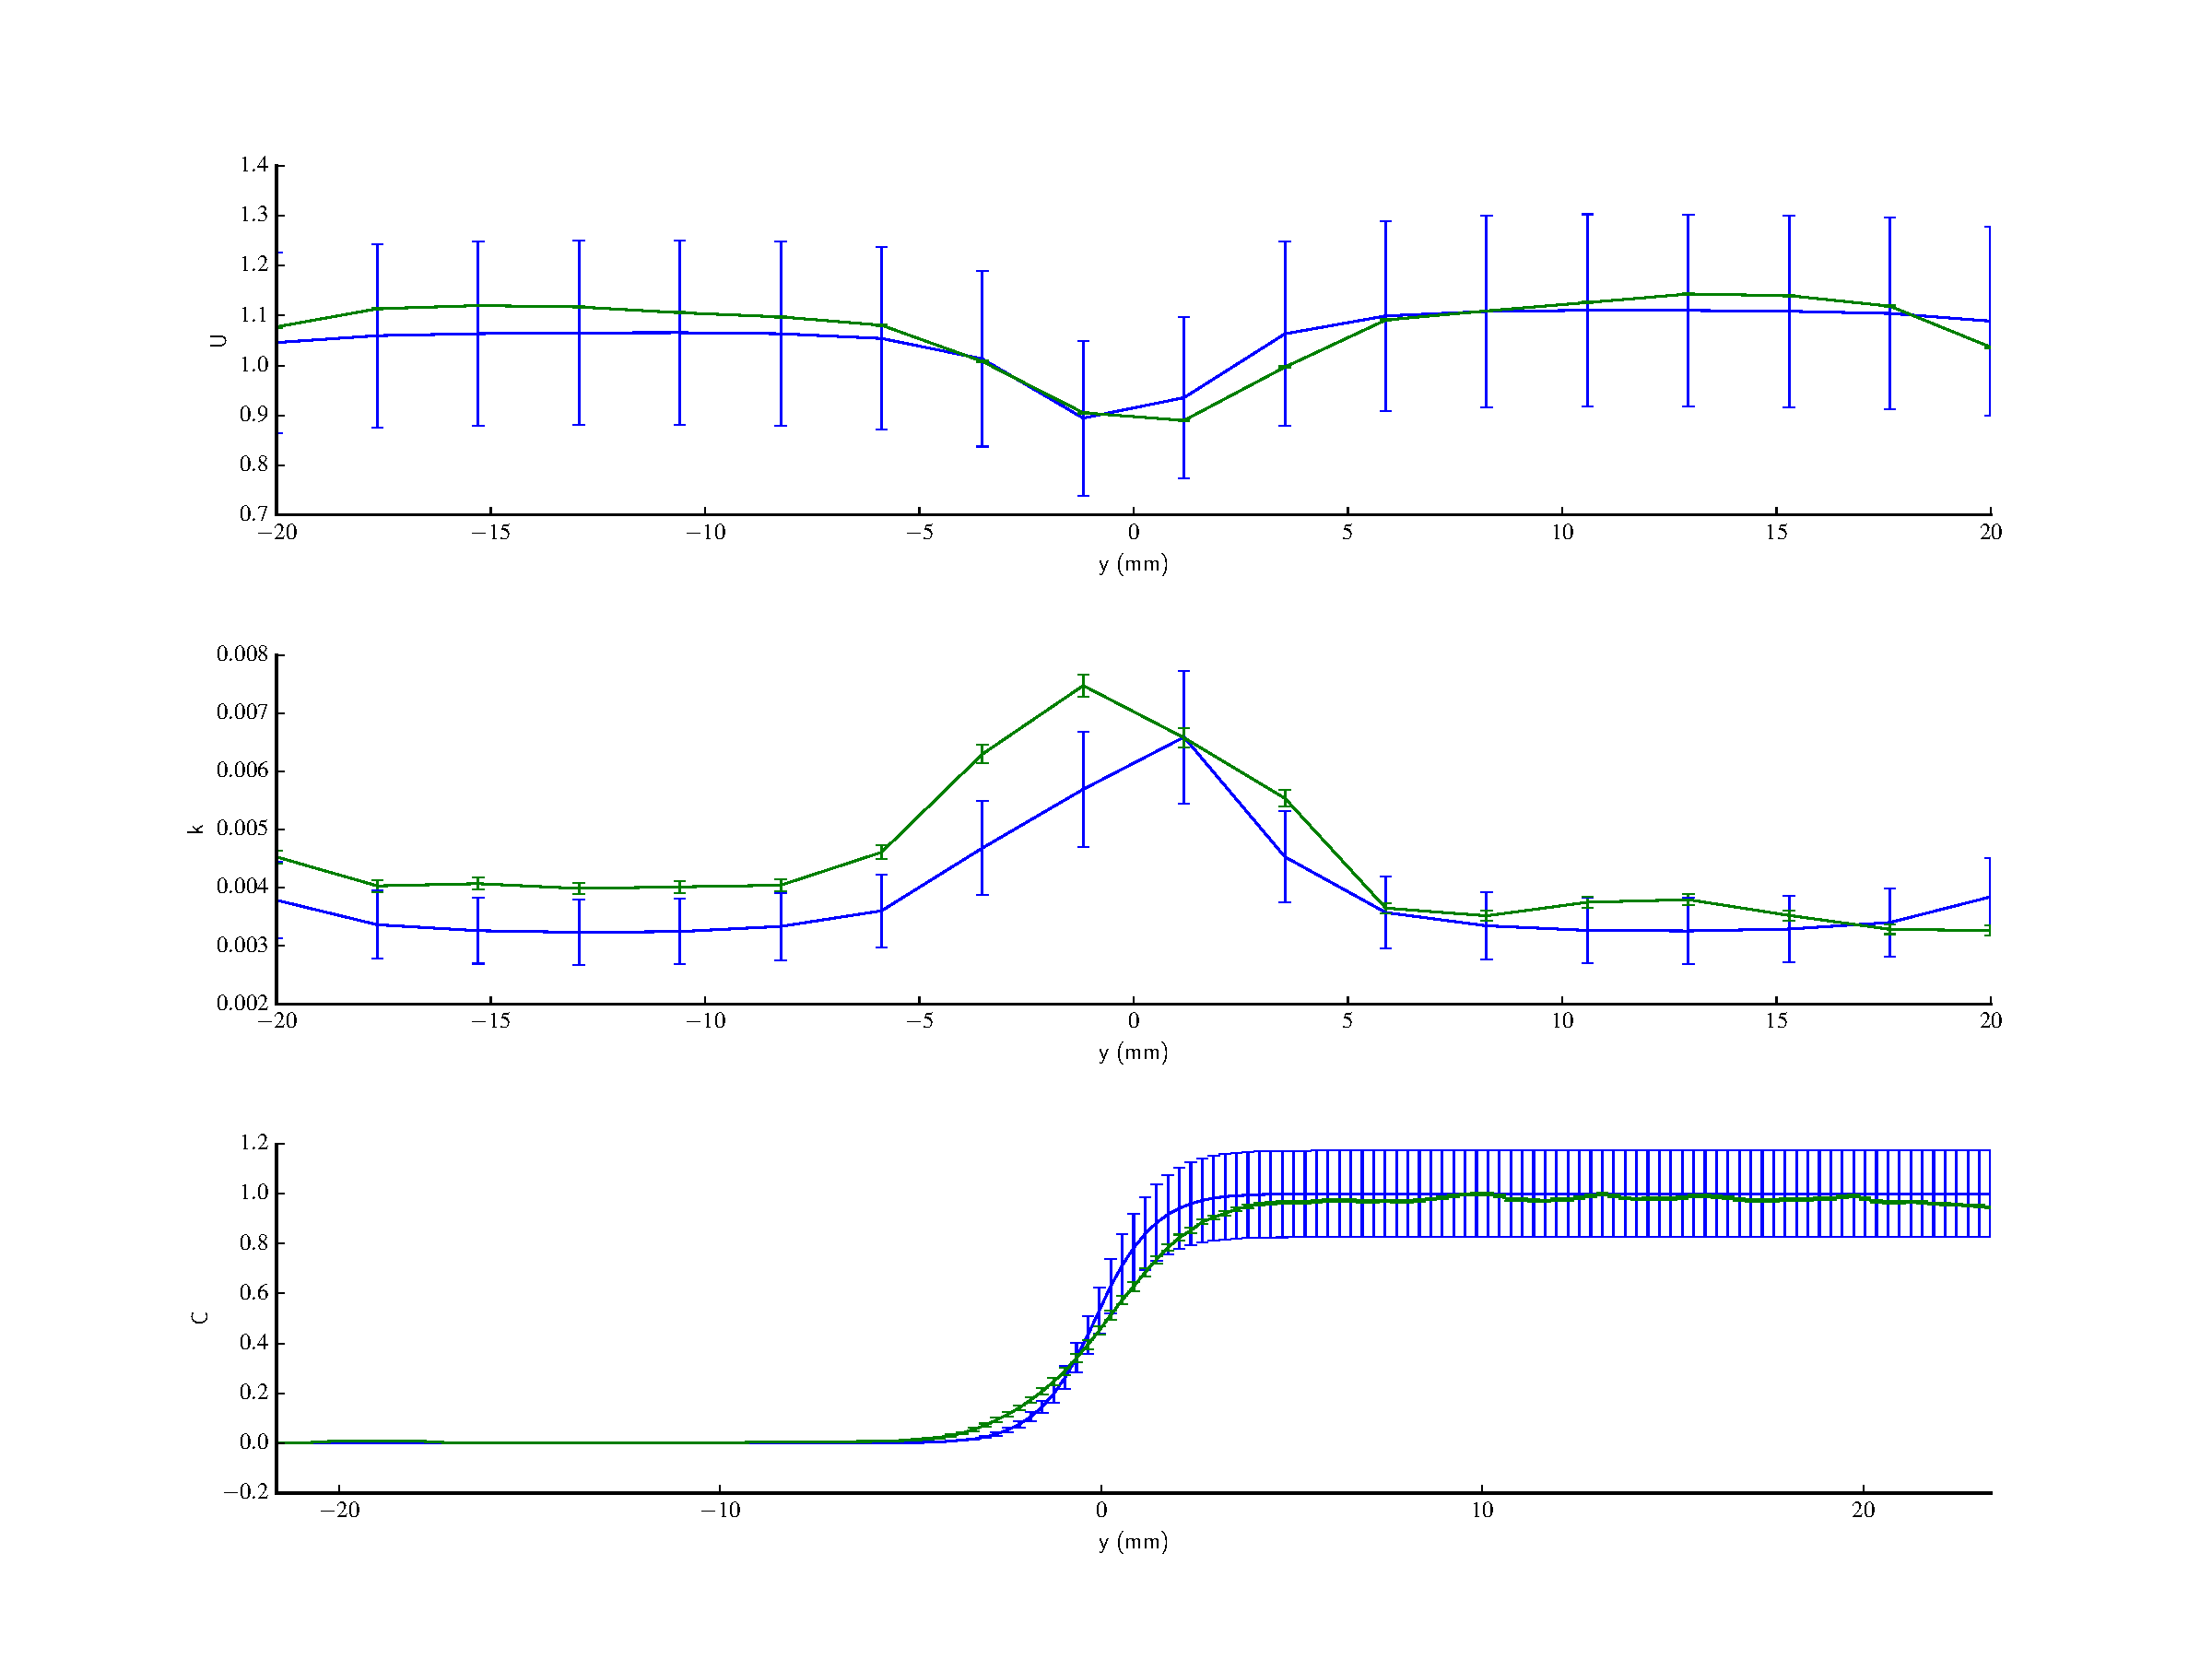
\includegraphics[width=\textwidth]{three_050.pdf}
			\caption{The velocity, turbulent kinetic energy and concentration profiles at \SI{50}{mm} downstream. }
		\end{figure}
		\begin{figure}[h]
			\centering
			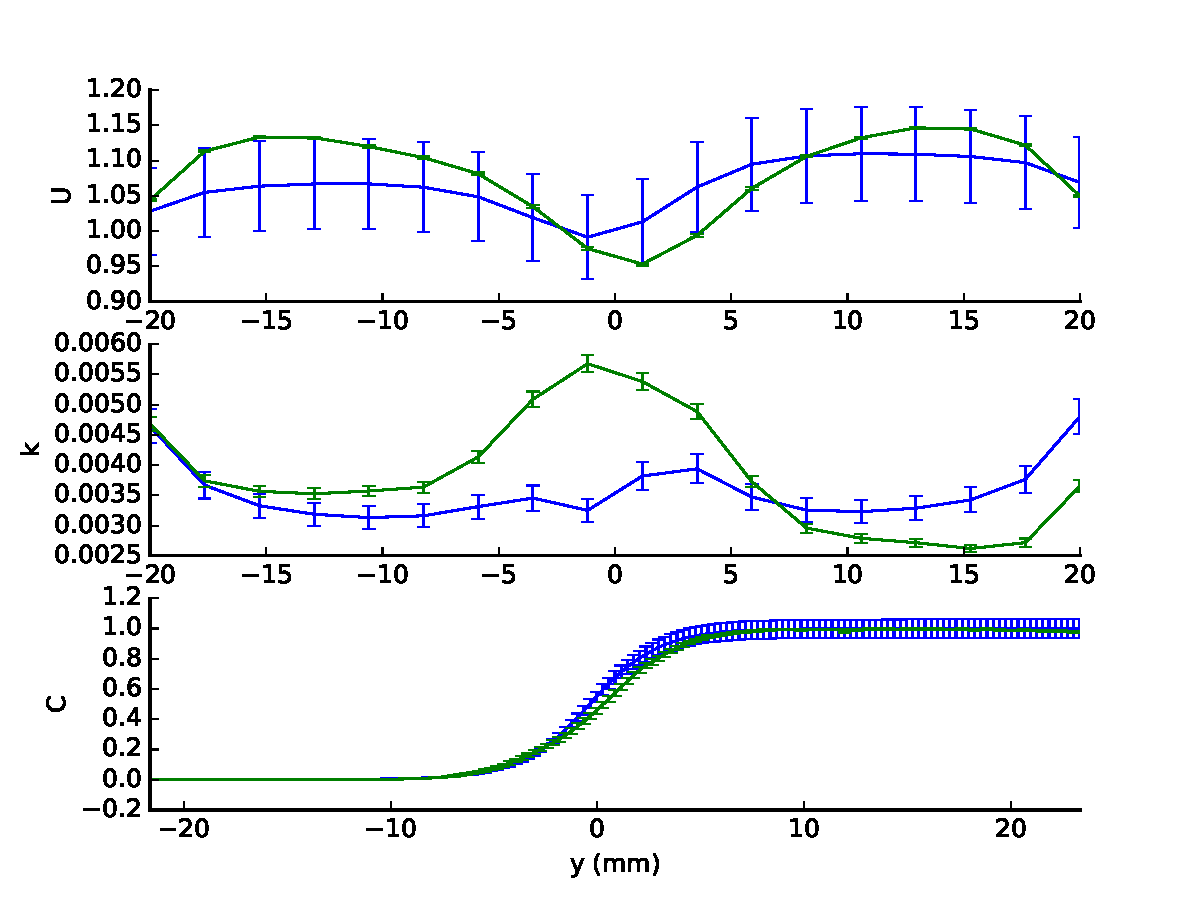
\includegraphics[width=\textwidth]{three_150.pdf}
			\caption{The velocity, turbulent kinetic energy and concentration profiles at \SI{150}{mm} downstream. }
		\end{figure}
		\begin{figure}[h]
			\centering
			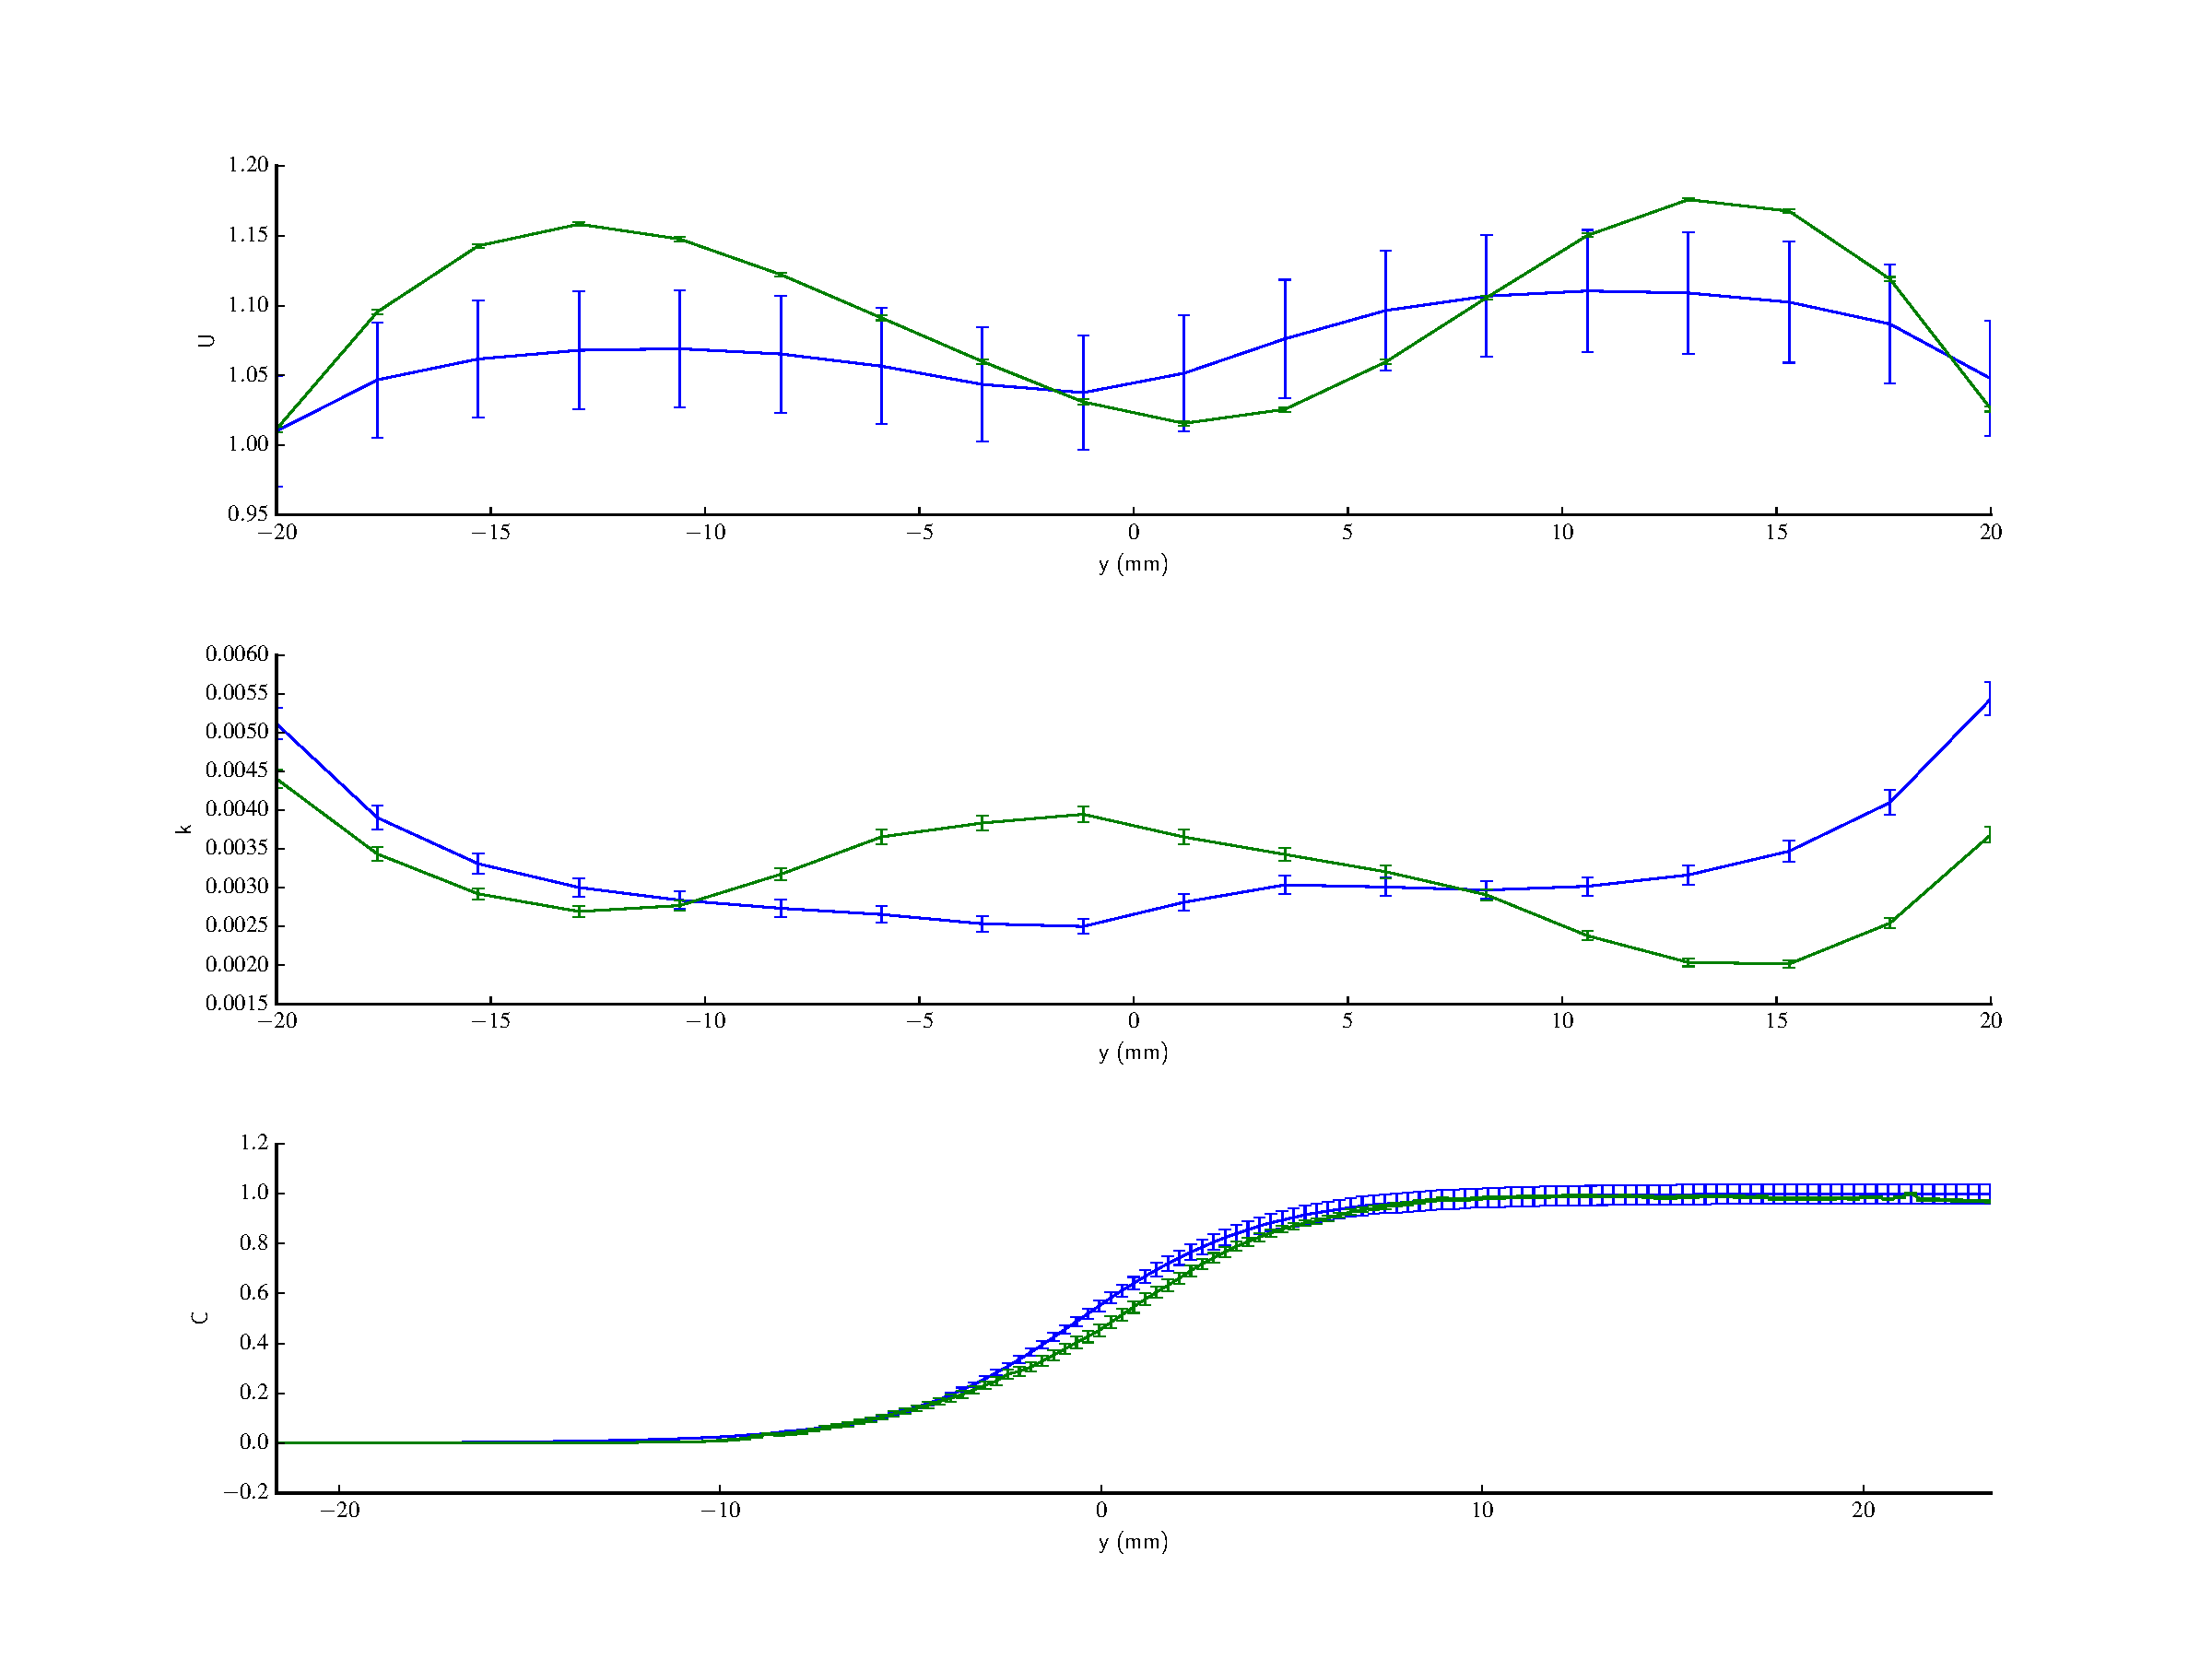
\includegraphics[width=\textwidth]{three_250.pdf}
			\caption{The velocity, turbulent kinetic energy and concentration profiles at \SI{250}{mm} downstream. }
		\end{figure}
		\begin{figure}[h]
			\centering
			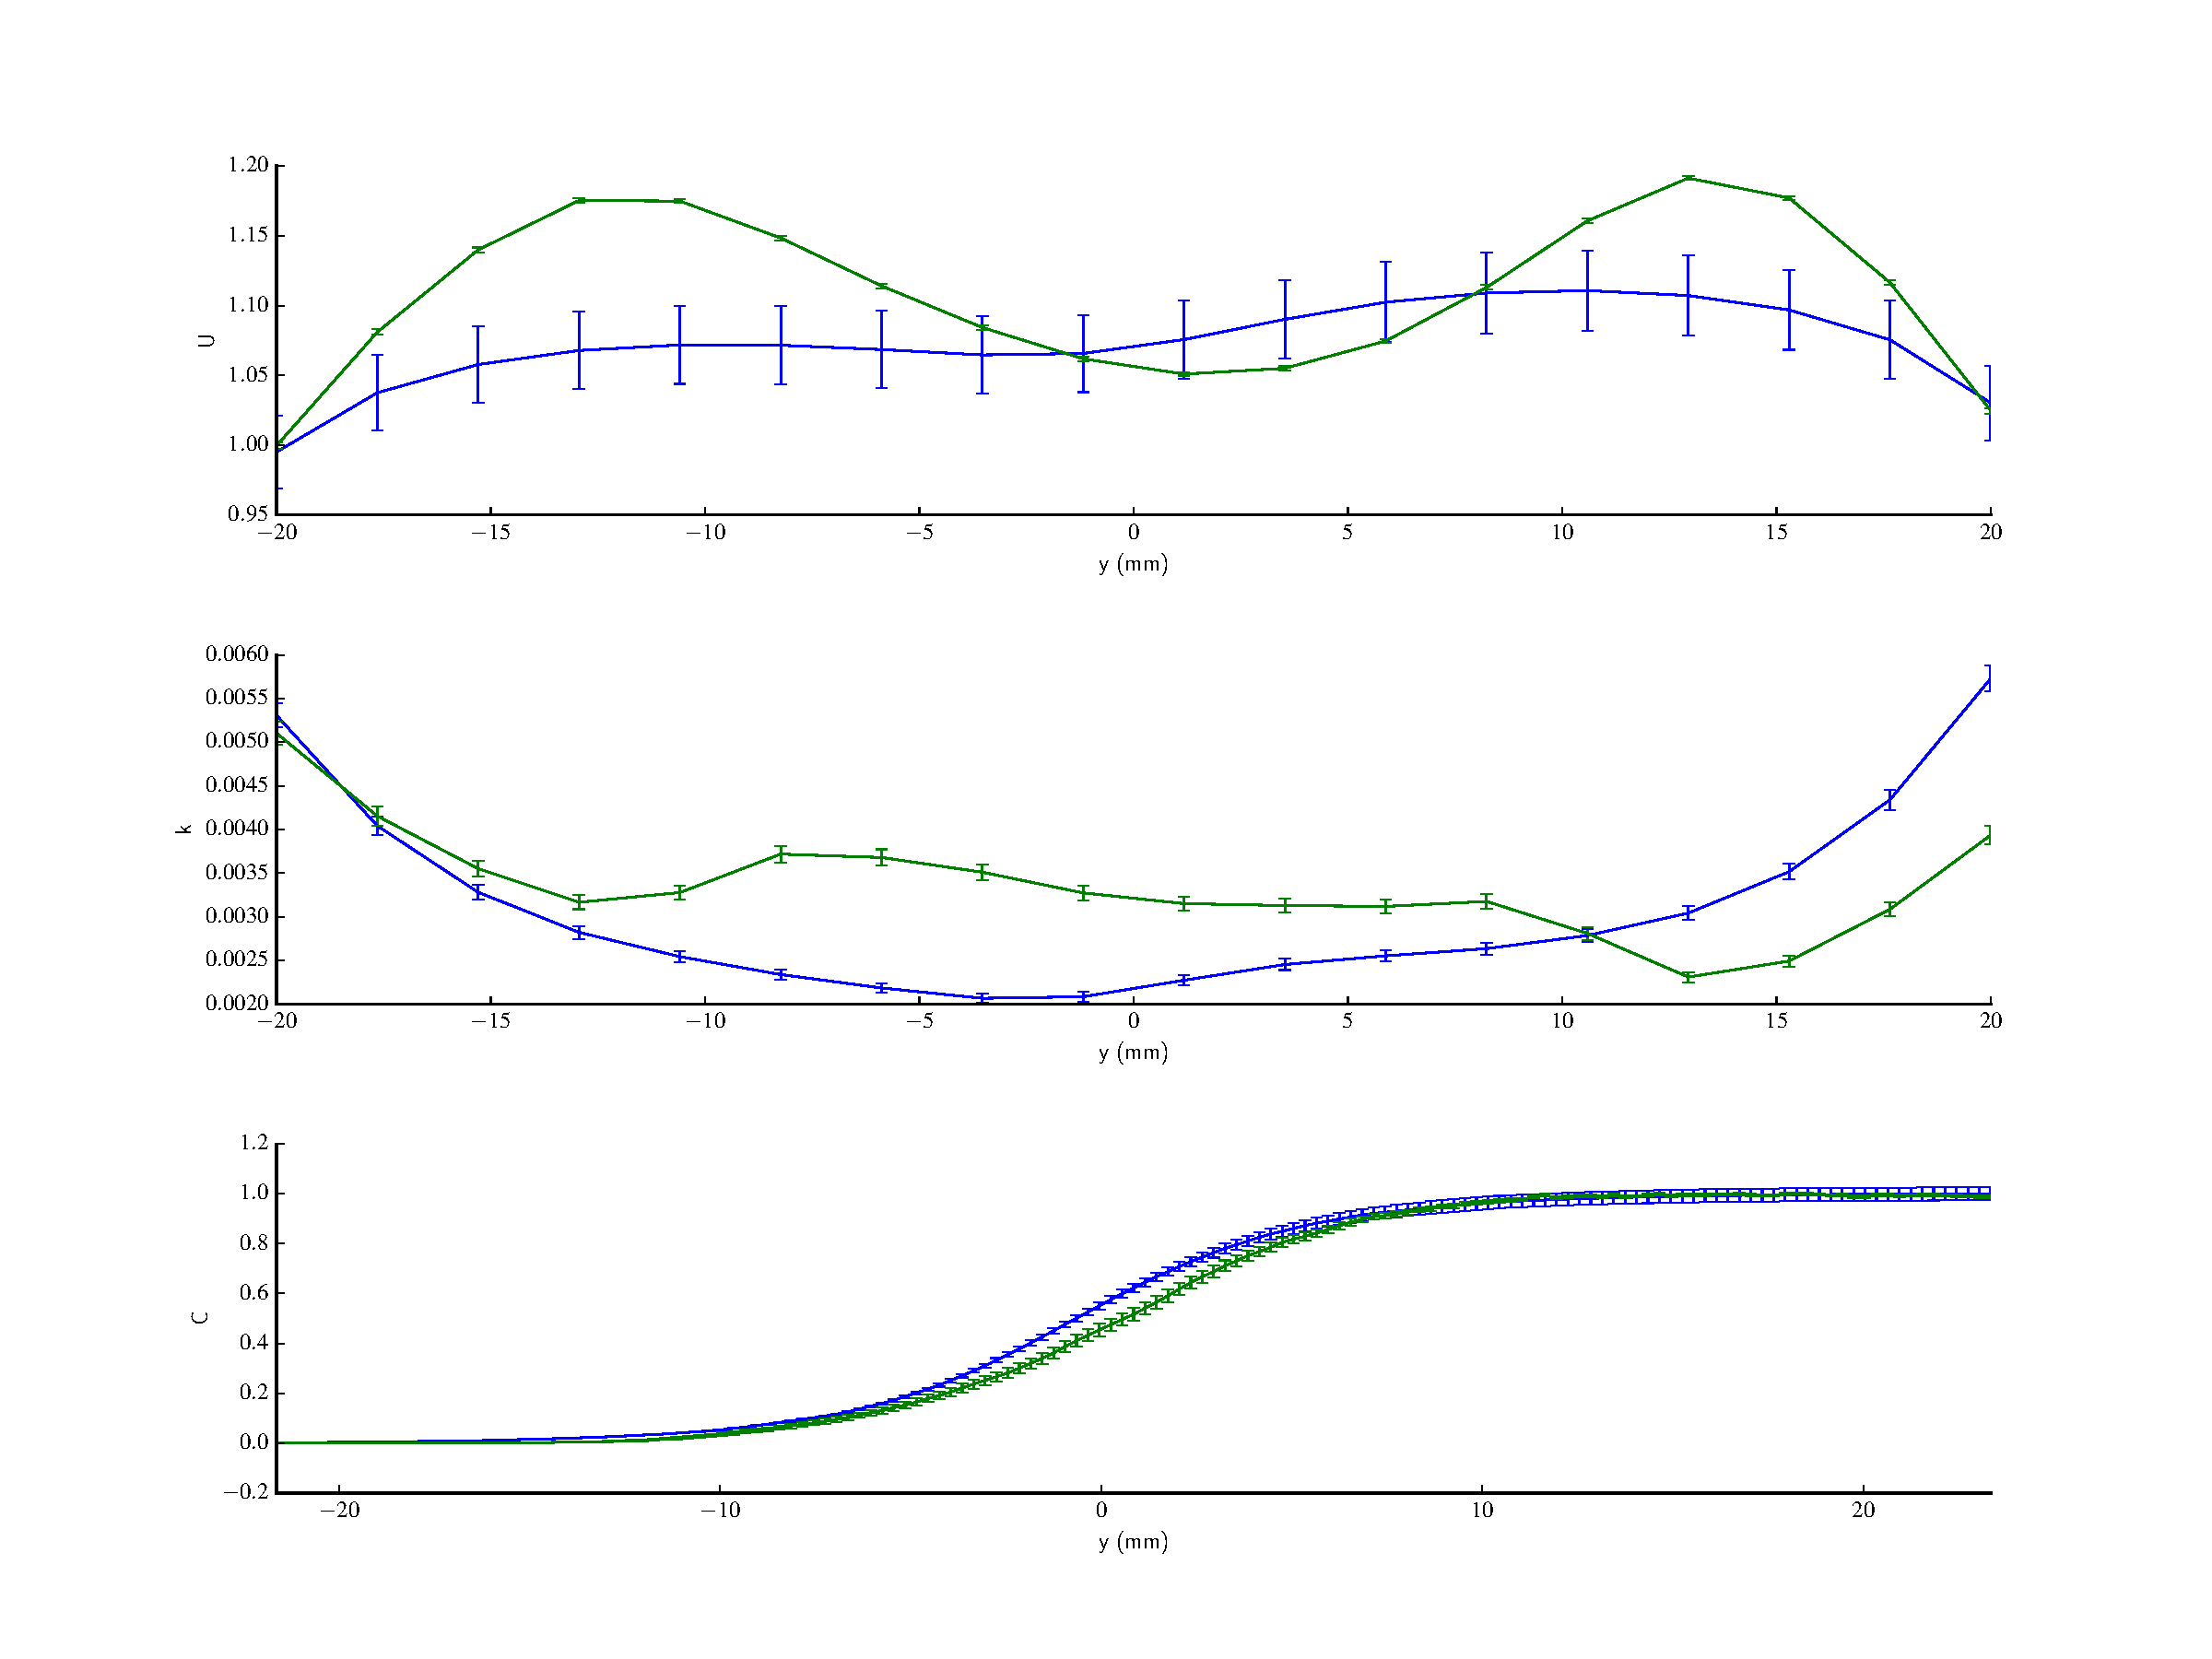
\includegraphics[width=\textwidth]{three_350.pdf}
			\caption{The velocity, turbulent kinetic energy and concentration profiles at \SI{350}{mm} downstream. }
		\end{figure}
		\begin{figure}[h]
			\centering
			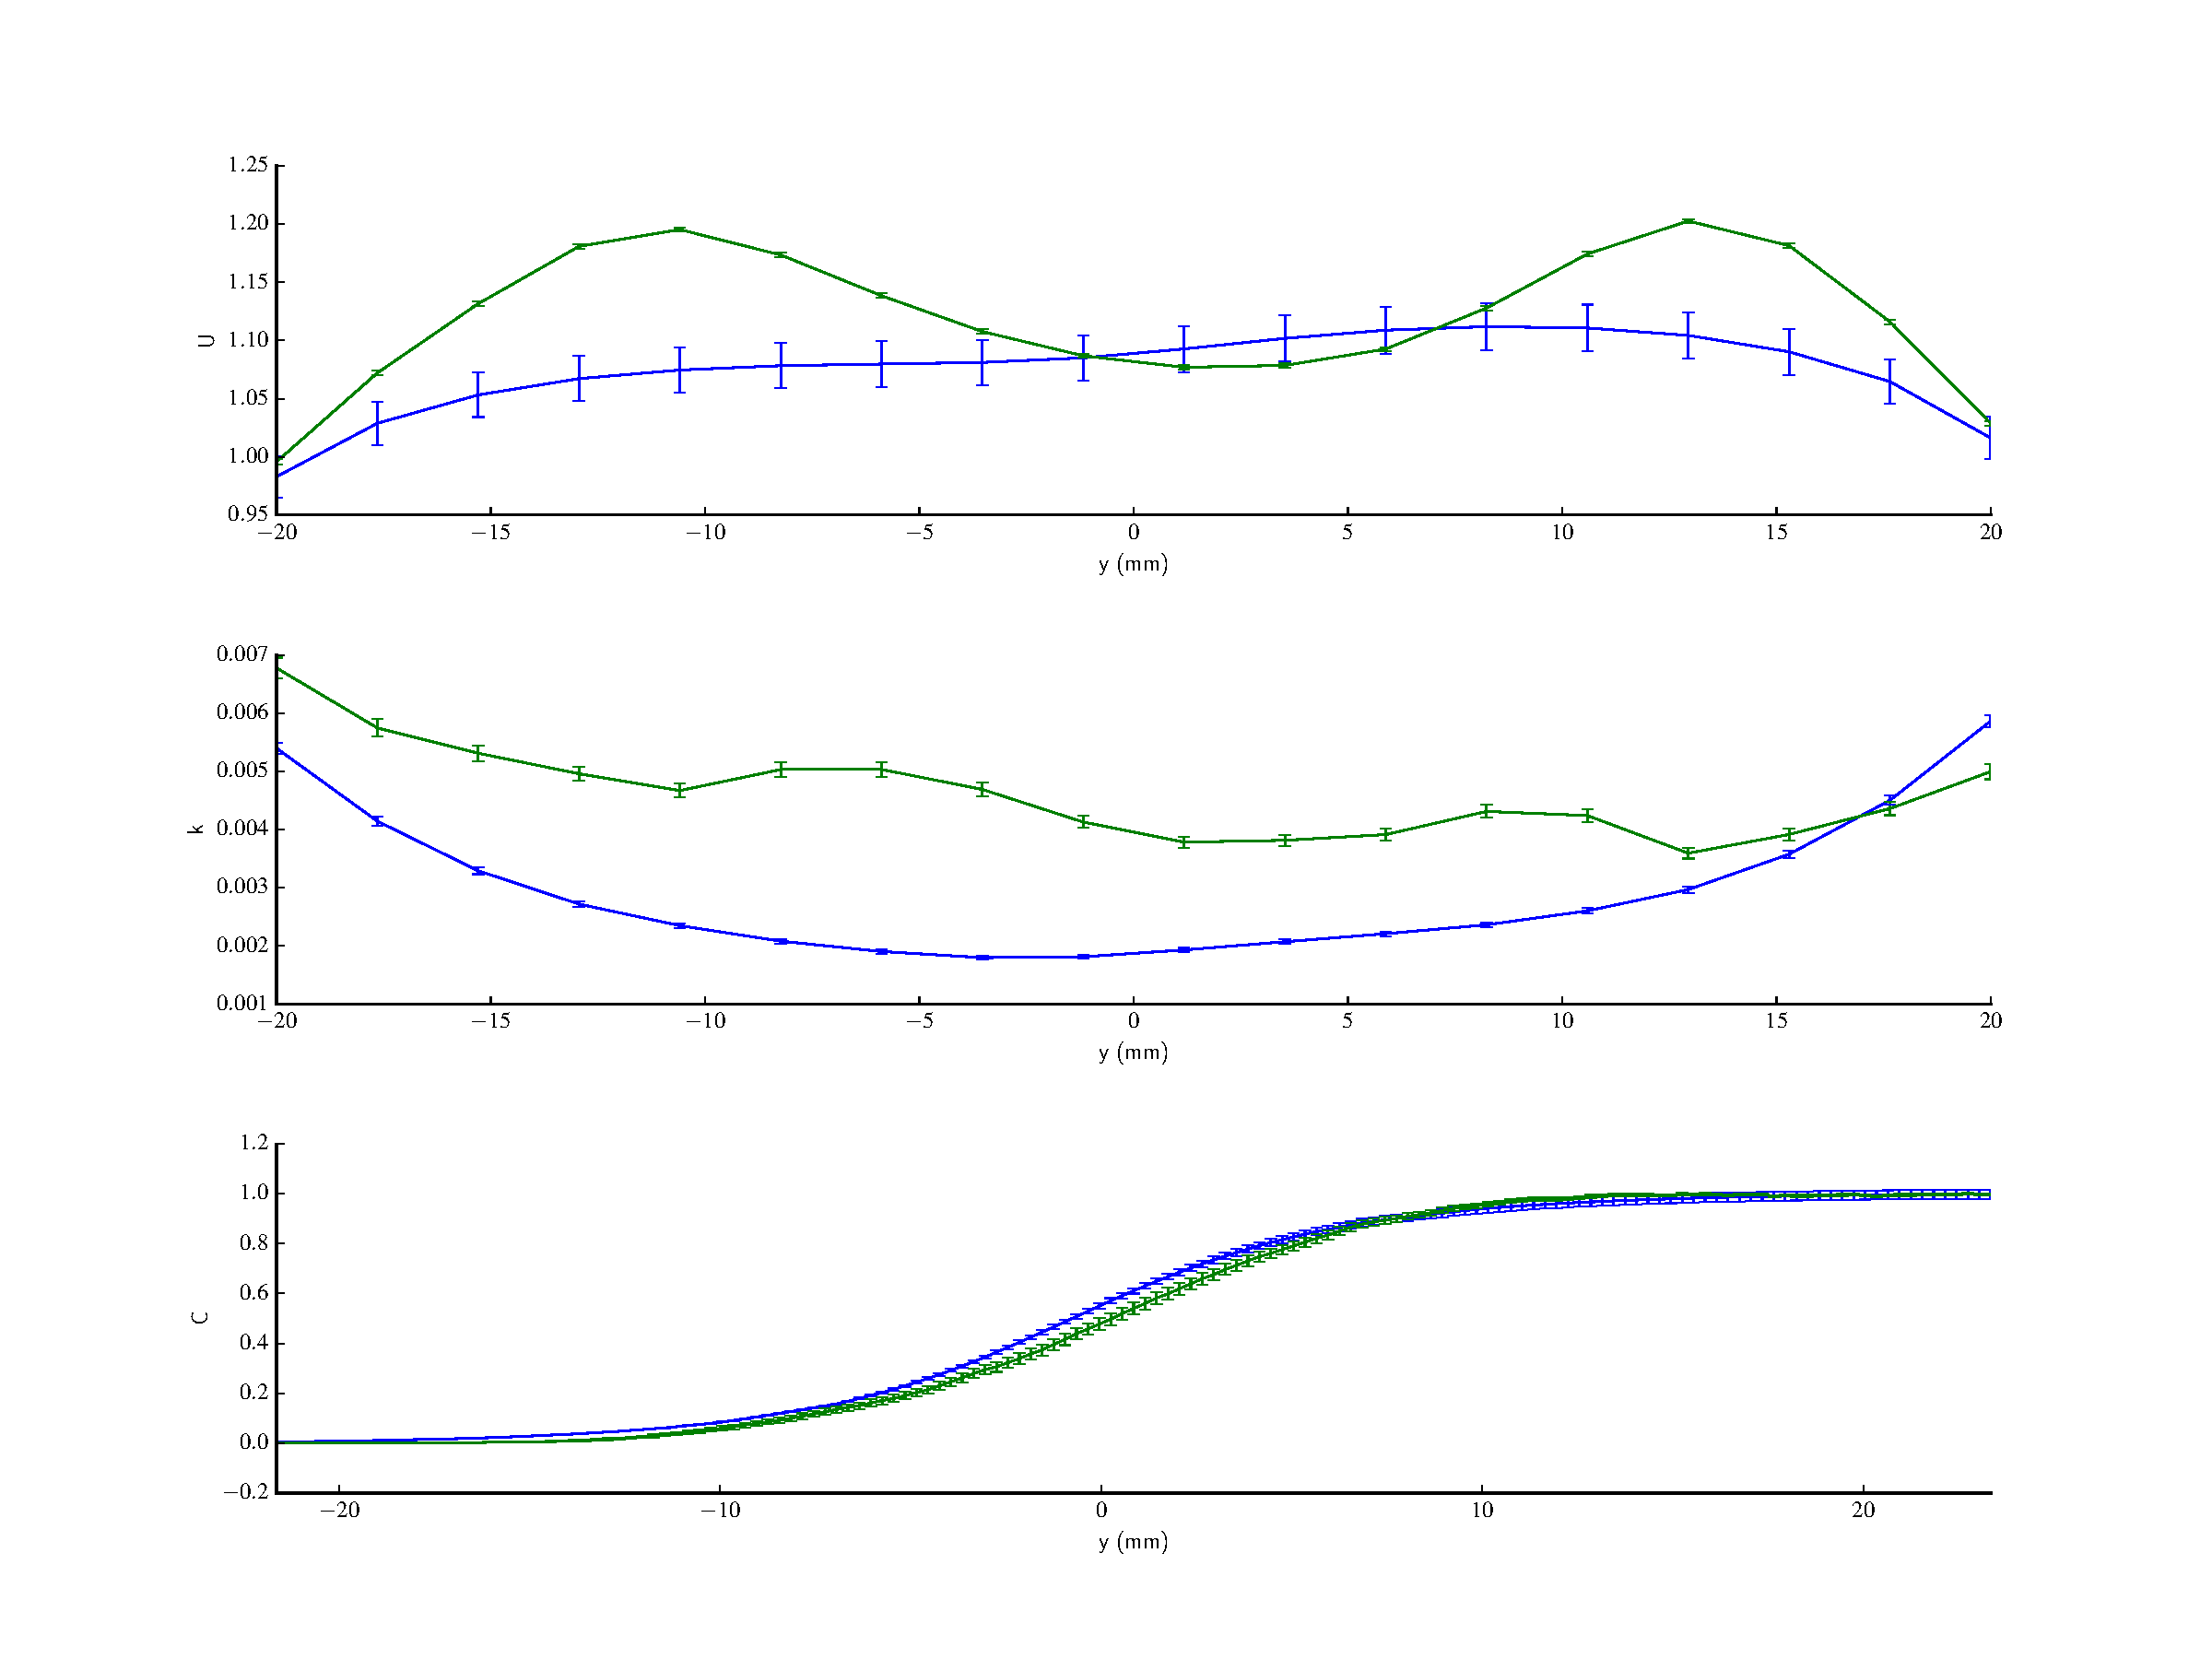
\includegraphics[width=\textwidth]{three_450.pdf}
			\caption{The velocity, turbulent kinetic energy and concentration profiles at \SI{450}{mm} downstream. }
		\end{figure}

\end{appendices}

\end{document} % --------------------------------------------------